\documentclass{article}

\usepackage{SIunits}
\usepackage{graphicx}
\usepackage{tikz}
\usepackage{pgfplots}

\usepgfplotslibrary{dateplot}
\usepgfplotslibrary{units}
\pgfplotsset{compat=1.14}

\begin{document}
\begin{tikzpicture}

\node (galileo) at (0,0) {
	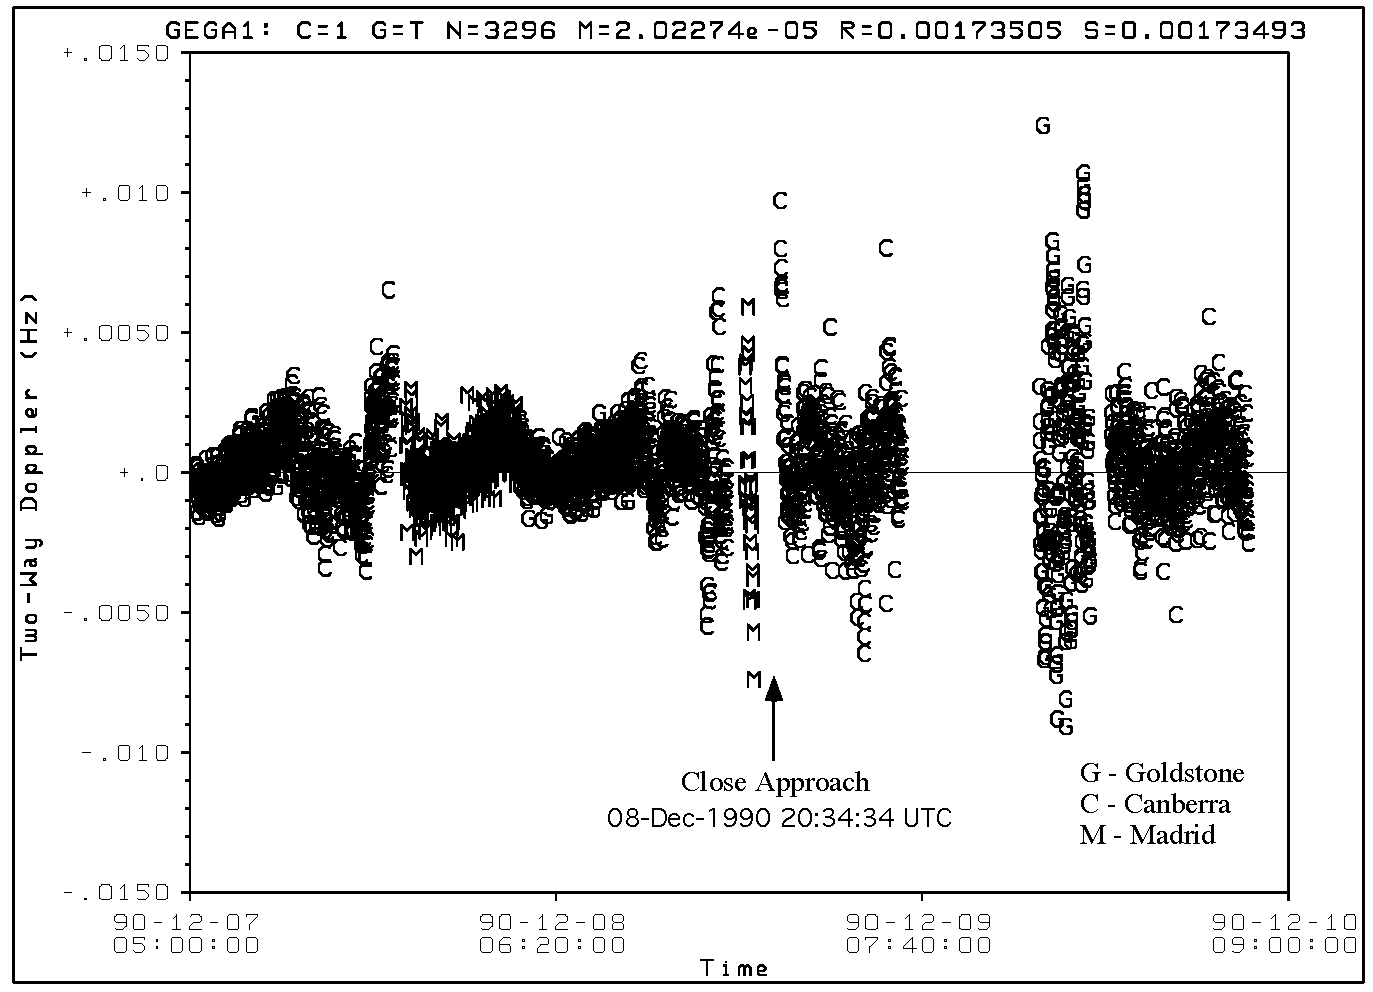
\includegraphics[width = 7.47cm] {Antreasian/fig3_g1dop_post_wlabels.pdf}
	};

\node (jplh) at (0.20, 0.05) {%
	\begin{tikzpicture}[xscale=0.8725,yscale=0.802]
	\footnotesize
	\begin{axis}[
		scaled ticks=false,
		axis line style = {blue},
		date coordinates in=x,
		date ZERO=1990-12-07 05:00:00,
		tick align = inside,
		xtick pos = left,
		xmin ={1990-12-07 05:00:00},
		xmax ={1990-12-10 09:00:00},
		xticklabel = {\tiny{\month-\day/\hour}},
		xticklabel style = {anchor = south, blue, align = center},
		yticklabel = \empty,
		ytick = \empty,
		restrict y to domain = -0.25:0.25,
		legend cell align = {left},
		legend style={
			at = {(0.05,0.90)},
			anchor = west,
			draw = none,
			font = \tiny,
			fill = white
			}
		]
		\addplot [thick, mark = none, red]
			table [x index=0, y index=8, col sep=tab, skip first n=1]
			{galileo_canberra.t}
		;
		\addlegendentry[red, align = left] {Canberra};

		\addplot [thick, mark = none, blue]
			table [x index=0, y index=8, col sep=tab, skip first n=1]
			{galileo_goldstone.t}
		;
		\addlegendentry[blue, align = left] {Madrid};

		\addplot [thick, mark = none, teal]
			table [x index=0, y index=8, col sep=tab, skip first n=1]
			{galileo_madrid.t}
		;
		\addlegendentry[teal, align = left] {Goldstone};
	\end{axis}
	\end{tikzpicture}
};
\end{tikzpicture}
\end{document}
